\documentclass[10pt]{article}

\usepackage[a4paper,margin=0.65in]{geometry}
\usepackage{amsmath,amssymb}
\usepackage{graphicx}
\usepackage{booktabs}
\usepackage{array}
\usepackage{float}
\usepackage{hyperref}
\usepackage{enumitem}
\usepackage{xcolor}
\usepackage{tikz}
\usetikzlibrary{positioning,arrows.meta,shapes.geometric,fit,calc}

\setlist{nosep,leftmargin=*}
\renewcommand{\arraystretch}{1.2}
\setlength{\parindent}{0pt}
\setlength{\parskip}{2pt}
\graphicspath{{experiment7_figures/}}

\tikzset{
layer/.style={draw,rounded corners,minimum width=1.7cm,minimum height=0.65cm,align=center,fill=blue!10,font=\scriptsize},
smalllayer/.style={draw,rounded corners,minimum width=1.35cm,minimum height=0.58cm,align=center,fill=green!10,font=\scriptsize},
arrow/.style={-{Latex[length=2mm]},thin}
}

\begin{document}

\begin{center}
{\large\textbf{Shiv Nadar University Chennai}}\\[2mm]
{\normalsize\textbf{CS3807 -- Deep Learning Laboratory}}\\[2mm]
{\large\textbf{Experiment 7}}\\[1mm]
{\normalsize\textbf{End-to-End Study of Autoencoders, Convolutional}}\\
{\normalsize\textbf{Autoencoders, Denoising Autoencoders and Variational Autoencoders}}
\end{center}

\vspace{3mm}
\begin{tabular}{|p{3.4cm}|p{9.0cm}|p{1.4cm}|}
\hline
Degree \& Branch & B.Tech Artificial Intelligence \& Data Science & Semester V\\
\hline
Subject Code \& Name & CS3807 -- Deep Learning Laboratory & AY: 2026--27\\
\hline
\end{tabular}

\section*{1. Objective}
The objective of this experiment is to develop an end-to-end understanding of autoencoders and their variants for image representation, reconstruction, denoising and generative modeling. The experiment progresses from a fully connected autoencoder to a convolutional autoencoder, a denoising convolutional autoencoder and finally a variational autoencoder (VAE). The learned latent representations are visualized and the models are evaluated using reconstruction metrics.

\section*{2. Learning Outcomes}
After completing this experiment, the following were studied and implemented:
\begin{itemize}
\item encoder--latent--decoder structure of an autoencoder;
\item image preparation for reconstruction learning;
\item fully connected and convolutional autoencoders;
\item controlled image corruption and denoising;
\item MSE, MAE and SSIM for reconstruction evaluation;
\item deterministic and probabilistic latent representations;
\item the VAE reparameterization trick and KL-divergence loss;
\item latent-space visualization, sampling and interpolation; and
\item reconstruction-error analysis and high-error image inspection.
\end{itemize}

\section*{3. Dataset and Experimental Setup}
\textbf{Dataset: MNIST Handwritten Digit Dataset.} MNIST contains grayscale handwritten digits from 0 to 9. Each image has spatial dimensions $28\times28\times1$. The laboratory execution used a fixed subset of 10,000 training images and 2,000 test images, as recommended by the experiment manual. Pixel values were normalized from $[0,255]$ to $[0,1]$. Labels were not supplied as reconstruction targets; the input image itself was used as the target.

\begin{center}
\begin{tabular}{|l|l|}
\hline
Training images & 10,000\\
Test images & 2,000\\
Image size & $28\times28\times1$\\
Flattened size & 784\\
Batch size & 128\\
FC/CAE epochs & 20\\
VAE epochs & 30\\
Optimizer & Adam\\
Learning rate & $10^{-3}$\\
\hline
\end{tabular}
\end{center}

The TensorFlow runtime reported version 2.20.0 and detected one GPU. The same train/test data protocol was maintained across the reconstruction models.

\section*{4. Overall Experimental Pipeline}
\begin{center}
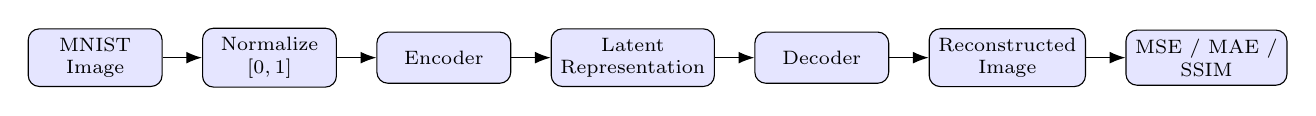
\begin{tikzpicture}[node distance=5mm]
\node[layer](a){MNIST\\Image};
\node[layer,right=of a](b){Normalize\\$[0,1]$};
\node[layer,right=of b](c){Encoder};
\node[layer,right=of c](d){Latent\\Representation};
\node[layer,right=of d](e){Decoder};
\node[layer,right=of e](f){Reconstructed\\Image};
\node[layer,right=of f](g){MSE / MAE /\\SSIM};
\foreach \x/\y in {a/b,b/c,c/d,d/e,e/f,f/g} \draw[arrow](\x)--(\y);
\end{tikzpicture}
\end{center}

Four related studies were performed: fully connected AE, convolutional AE, denoising CAE and VAE. An additional latent-dimension study was performed for the fully connected autoencoder.

\section*{5. Autoencoder Theory}
An autoencoder learns a reconstruction mapping
\[
z=f_{\theta}(x), \qquad \hat{x}=g_{\phi}(z).
\]
The reconstruction objective is to minimize the difference between $x$ and $\hat{x}$. For squared reconstruction error,
\[
L_{rec}=\frac{1}{N}\sum_{i=1}^{N}\lVert x_i-\hat{x}_i\rVert^2.
\]
The latent vector is a compressed representation of the input.
\section*{6. Github Link: }
\url{https://github.com/PranavVarshin/DeepLearning/tree/main/Lab-7}
\section*{7. Fully Connected Autoencoder}
The images were flattened from $28\times28$ to 784 values. The implemented architecture was
\[
784\rightarrow128\rightarrow32\rightarrow d_z\rightarrow32\rightarrow128\rightarrow784,
\]
with ReLU activations in hidden layers and sigmoid activation at the output. The main model used $d_z=16$.

The model was trained for 20 epochs using Adam with learning rate $10^{-3}$, batch size 128 and binary cross-entropy loss. Ten percent of the training subset was used for validation.

\subsection*{7.1 Reconstruction and Convergence}
Figure~\ref{fig:fcrecon} shows original images, FC-AE reconstructions and absolute reconstruction errors.

\begin{figure}[H]\centering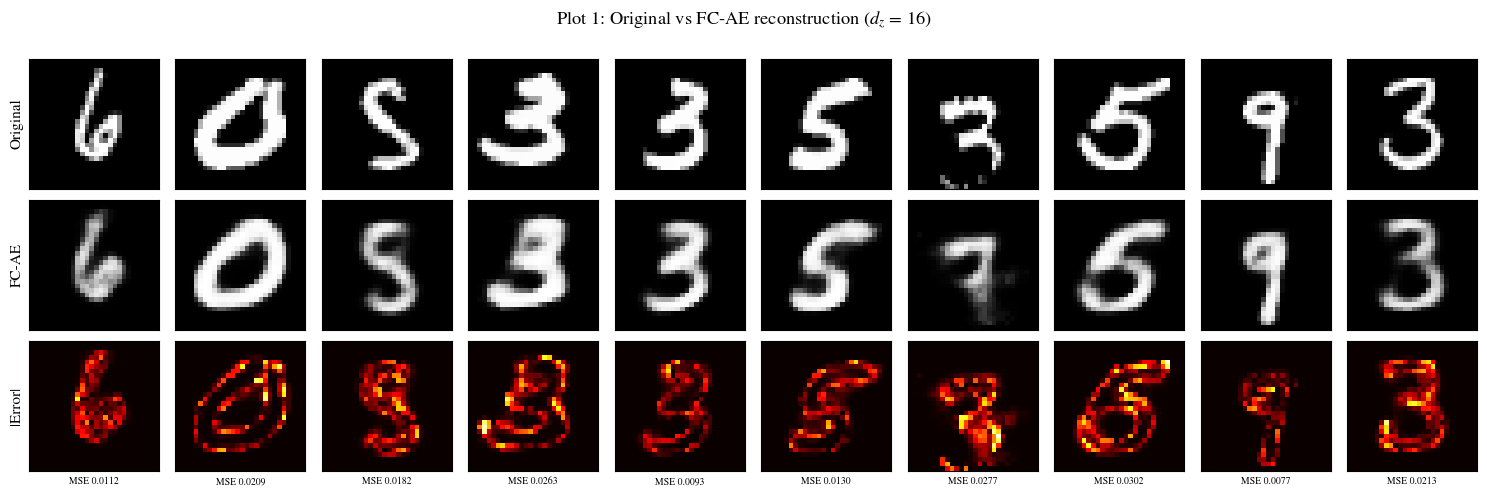
\includegraphics[width=\textwidth]{cell6_img0.png}\caption{Original images, FC-AE reconstructions and absolute error maps.}\label{fig:fcrecon}\end{figure}

The final training loss was 0.1217 and validation loss was 0.1226, giving a small gap of 0.0009. The curves decrease steadily over the 20 epochs, indicating convergence without a clear validation-loss divergence.

\begin{figure}[H]\centering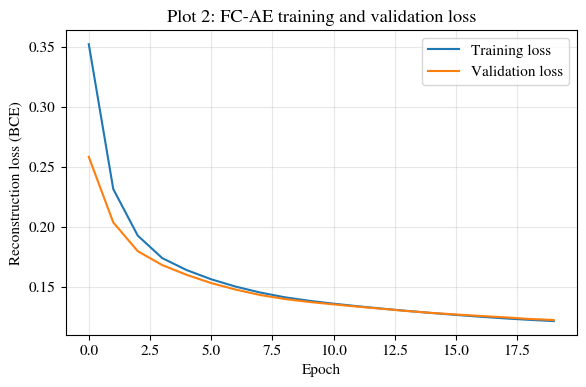
\includegraphics[width=0.72\textwidth]{cell7_img1.png}\caption{FC-AE training and validation reconstruction loss.}\label{fig:fcloss}\end{figure}

\subsection*{7.2 Test Metrics}
\begin{center}
\begin{tabular}{|l|r|}
\hline
Test MSE & 0.01992\\
Test MAE & 0.05442\\
Mean SSIM & 0.7749\\
Parameters & 211,040\\
Training time & 12.0 s\\
\hline
\end{tabular}
\end{center}

\subsection*{7.3 Latent-Dimension Study}
The FC-AE was repeated with $d_z\in\{2,8,16,32\}$.
\begin{center}
\begin{tabular}{rrrr}
\toprule
Latent dimension & MSE & SSIM & Parameters\\
\midrule
2 & 0.04718 & 0.4729 & 210130\\
8 & 0.02595 & 0.7107 & 210520\\
16 & 0.02025 & 0.7712 & 211040\\
32 & 0.01919 & 0.7814 & 212080\\
\bottomrule
\end{tabular}
\end{center}

\begin{figure}[H]\centering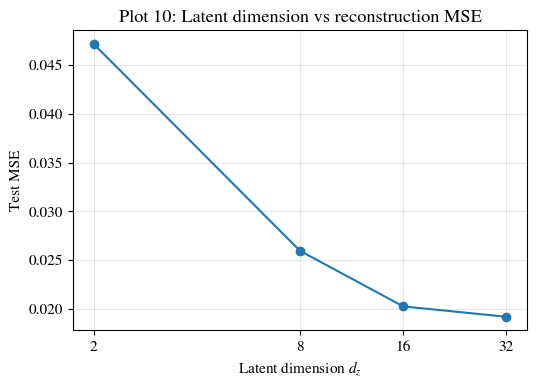
\includegraphics[width=0.75\textwidth]{cell10_img1.png}\caption{Latent dimension versus reconstruction MSE and representative reconstructions.}\label{fig:latentdim}\end{figure}

Increasing the latent dimension improved reconstruction quality. The largest change occurred from 2 to 8 dimensions, while the improvement from 16 to 32 was comparatively small. This demonstrates the compression--reconstruction trade-off.

\section*{8. Convolutional Autoencoder}
The convolutional autoencoder preserved the spatial structure of the images. The implemented architecture was
\[
\text{Conv32}\rightarrow\text{MaxPool}\rightarrow\text{Conv64}\rightarrow\text{MaxPool}\rightarrow\text{Conv64}
\]
for the encoder, followed by upsampling, convolution and a sigmoid output for the decoder. The latent feature map contained $7\times7\times64=3136$ values.

The model used the same 20-epoch training protocol as the FC-AE.

\begin{figure}[H]\centering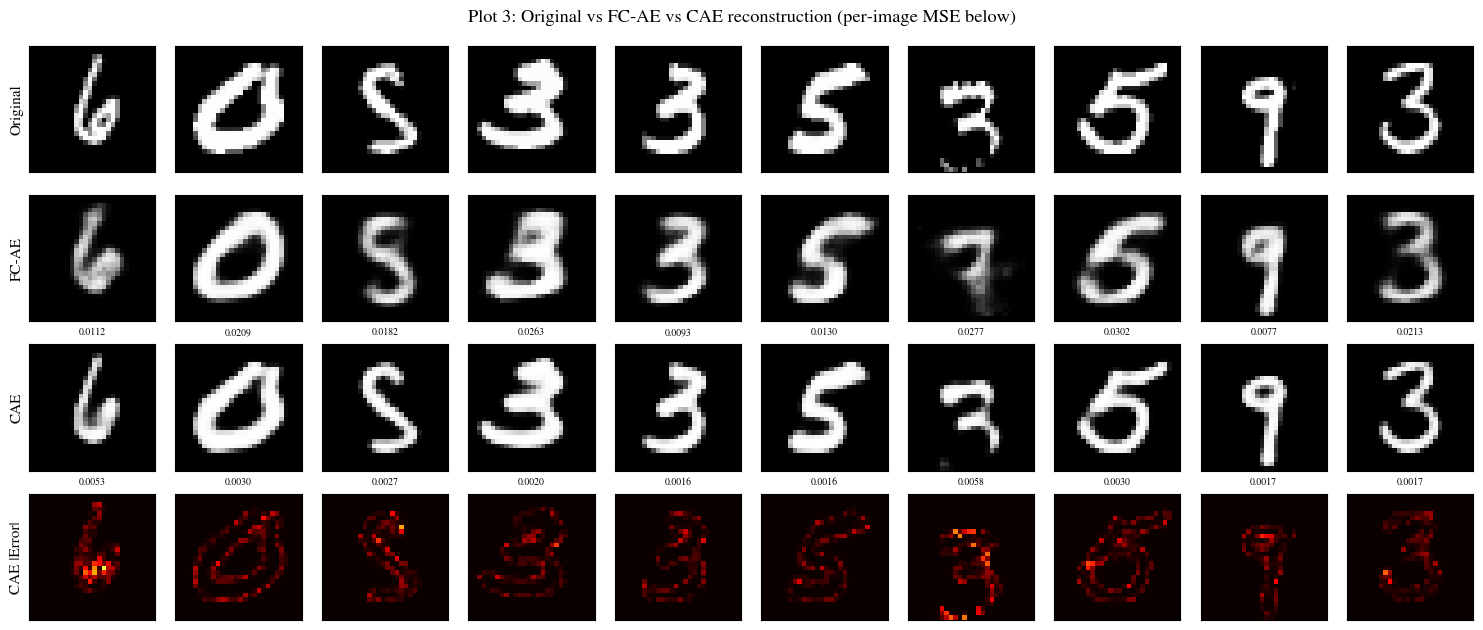
\includegraphics[width=0.95\textwidth]{cell15_img0.png}\caption{FC-AE versus convolutional AE reconstruction comparison.}\label{fig:caecomp}\end{figure}

\begin{center}
\begin{tabular}{|l|r|r|r|r|}
\hline
Model & MSE & MAE & SSIM & Parameters\\
\hline
FC Autoencoder & 0.01992 & 0.05442 & 0.7749 & 211040\\
Conv. Autoencoder & 0.00264 & 0.01554 & 0.9725 & 74497\\
\hline
\end{tabular}
\end{center}

The convolutional autoencoder reduced MSE by approximately 86.7\% relative to the FC-AE and increased SSIM by 0.1976. This is consistent with the benefit of preserving local spatial structure through convolution.

\section*{9. Denoising Convolutional Autoencoder}
A denoising autoencoder receives a corrupted image $\tilde{x}$ and learns to reconstruct the clean image $x$:
\[
\tilde{x}\rightarrow\text{Encoder}\rightarrow z\rightarrow\text{Decoder}\rightarrow\hat{x}.
\]
Two corruption types were tested.

\subsection*{9.1 Gaussian Noise}
Gaussian corruption was generated using
\[
\tilde{x}=x+n,\qquad n\sim\mathcal{N}(0,\sigma^2),
\]
with $\sigma\in\{0.1,0.2,0.3\}$. Values were clipped to $[0,1]$.

\subsection*{9.2 Salt-and-Pepper Noise}
For salt-and-pepper corruption, a proportion $p\in\{0.05,0.10,0.20\}$ of pixels was replaced with values close to 0 or 1.

The denoising CAEs used the same convolutional architecture and training protocol as the plain CAE. The headline denoising model used Gaussian noise with $\sigma=0.2$.

\begin{figure}[H]\centering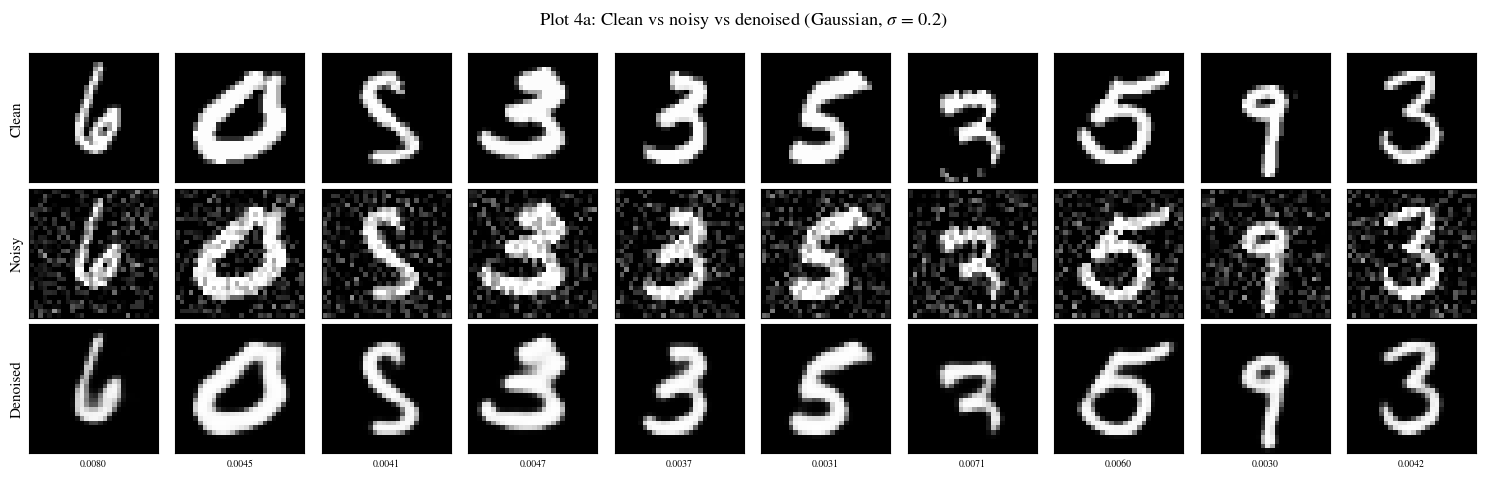
\includegraphics[width=0.95\textwidth]{cell20_img0.png}\caption{Clean, noisy and denoised MNIST images for Gaussian noise.}\label{fig:denoiseg}\end{figure}

\begin{figure}[H]\centering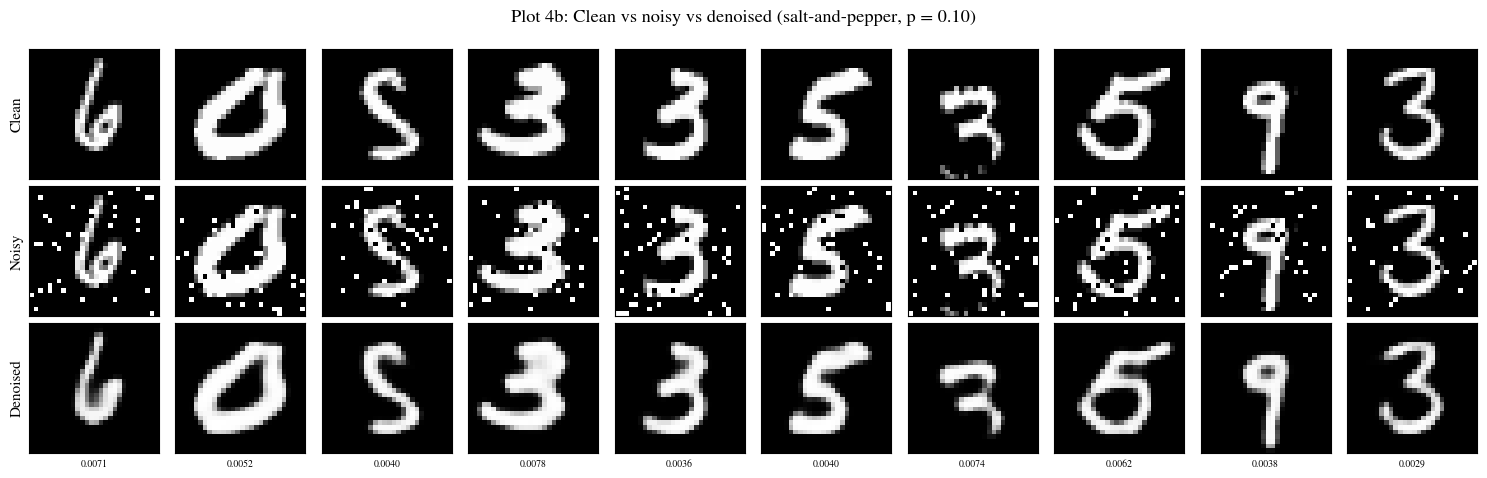
\includegraphics[width=0.95\textwidth]{cell20_img1.png}\caption{Clean, noisy and denoised MNIST images for salt-and-pepper noise.}\label{fig:denoisesp}\end{figure}

\subsection*{9.3 Denoising Results}
\begin{center}
\begin{tabular}{rrrr|rrr}
\toprule
\multicolumn{4}{c|}{Gaussian noise} & \multicolumn{3}{c}{Denoised output}\\
Level & MSE & MAE & SSIM & & &\\
\midrule
0.1 & 0.00315 & 0.01734 & 0.9649 & & &\\
0.2 & 0.00444 & 0.02111 & 0.9480 & & &\\
0.3 & 0.00659 & 0.02641 & 0.9222 & & &\\
\bottomrule
\end{tabular}
\end{center}

\begin{center}
\begin{tabular}{rrrr}
\toprule
Salt-and-pepper $p$ & MSE & MAE & SSIM\\
\midrule
0.05 & 0.00379 & 0.01871 & 0.9587\\
0.10 & 0.00516 & 0.02210 & 0.9441\\
0.20 & 0.00782 & 0.02850 & 0.9121\\
\bottomrule
\end{tabular}
\end{center}

\begin{figure}[H]\centering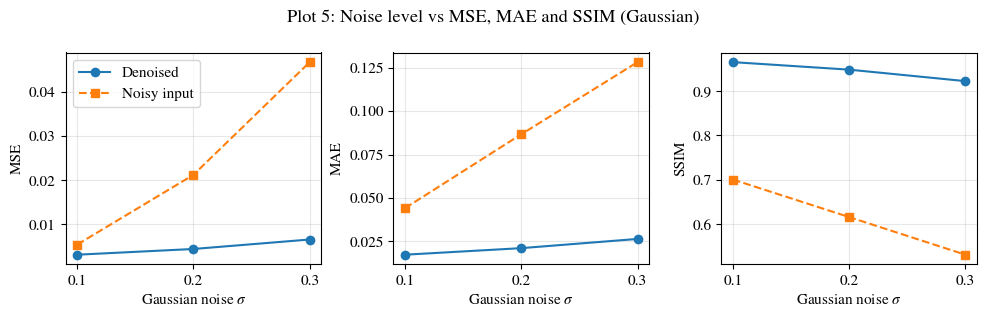
\includegraphics[width=0.88\textwidth]{cell21_img1.png}\caption{Gaussian noise level versus denoising reconstruction quality.}\label{fig:noiseg}\end{figure}

\begin{figure}[H]\centering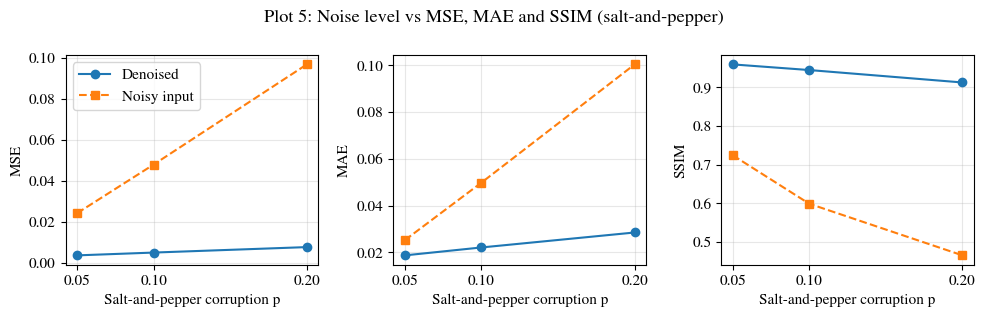
\includegraphics[width=0.88\textwidth]{cell21_img3.png}\caption{Salt-and-pepper noise level versus denoising reconstruction quality.}\label{fig:noisesp}\end{figure}

As corruption increased, denoising MSE and MAE increased while SSIM decreased. However, the denoised outputs remained substantially better than the corresponding noisy inputs, showing that the model recovered the major digit structure.

\section*{10. Variational Autoencoder}
Unlike a conventional autoencoder, the VAE learns a probability distribution in latent space:
\[
q_{\phi}(z|x)=\mathcal{N}\left(\mu(x),\operatorname{diag}(\sigma^2(x))\right).
\]
The encoder produced $\mu$ and $\log\sigma^2$ for a two-dimensional latent representation. Sampling used the reparameterization trick:
\[
z=\mu+\sigma\odot\epsilon,\qquad \epsilon\sim\mathcal{N}(0,I).
\]

The VAE used a convolutional encoder with two strided convolution layers, a dense layer and two latent heads. The decoder mapped a two-dimensional latent vector back to a $28\times28\times1$ image using a dense layer and transposed convolutions.

The loss consisted of reconstruction and KL-divergence terms:
\[
L_{VAE}=L_{rec}+L_{KL},
\]
where
\[
D_{KL}(q_{\phi}(z|x)\Vert p(z))=-\frac12\sum_j\left(1+\log\sigma_j^2-\mu_j^2-\sigma_j^2\right).
\]
The prior was $p(z)=\mathcal{N}(0,I)$.

The VAE was trained for 30 epochs with Adam, learning rate $10^{-3}$ and batch size 128. It contained 134,165 trainable parameters and required 26.9 seconds.

\begin{figure}[H]\centering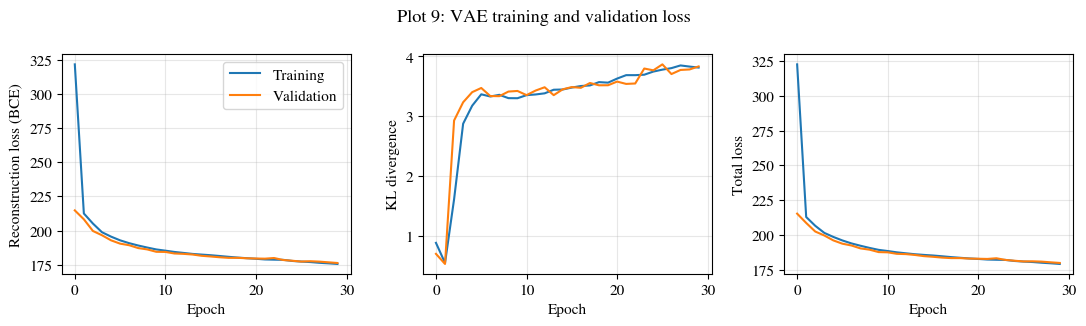
\includegraphics[width=0.90\textwidth]{cell26_img1.png}\caption{VAE reconstruction, KL and total training/validation losses.}\label{fig:vaeloss}\end{figure}

The final training reconstruction, KL and total losses were 175.55, 3.81 and 179.37 respectively. The corresponding validation values were 176.25, 3.83 and 180.08.

\subsection*{10.1 VAE Test Metrics}
\begin{center}
\begin{tabular}{|l|r|}
\hline
Reconstruction loss & 176.266\\
KL loss & 3.857\\
Total loss & 180.123\\
Test MSE & 0.05474\\
Test MAE & 0.12666\\
Mean SSIM & 0.3661\\
Parameters & 134,165\\
Training time & 26.9 s\\
\hline
\end{tabular}
\end{center}
\clearpage

\section*{11. VAE Latent Space and Generation}
The two-dimensional latent representation was visualized using the encoded means $(z_1,z_2)$. The VAE was not trained using labels; labels were used only to colour the visualization and calculate the auxiliary 5-NN statistic.

The mean of the encoded means was approximately $[-1.01,-0.016]$ and the standard deviations were approximately $[0.757,0.038]$. The mean encoded standard deviations were $[0.038,0.846]$. The KL loss per latent dimension was approximately $[3.813,0.044]$, with total KL loss 3.857.

\begin{figure}[H]\centering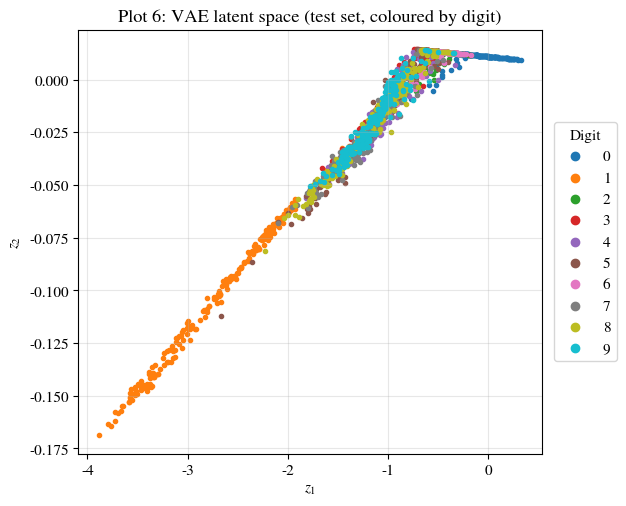
\includegraphics[width=0.72\textwidth]{cell29_img1.png}\caption{Two-dimensional VAE latent-space visualization.}\label{fig:vaelatent}\end{figure}

The auxiliary 5-NN digit accuracy in the 2-D latent space was 0.412, indicating substantial overlap among digit classes in the learned representation.
\clearpage
\subsection*{11.1 Random Generation}
New latent vectors were sampled from $\mathcal{N}(0,I)$ and passed through the decoder without an input image. At least 25 samples were generated.

\begin{figure}[H]\centering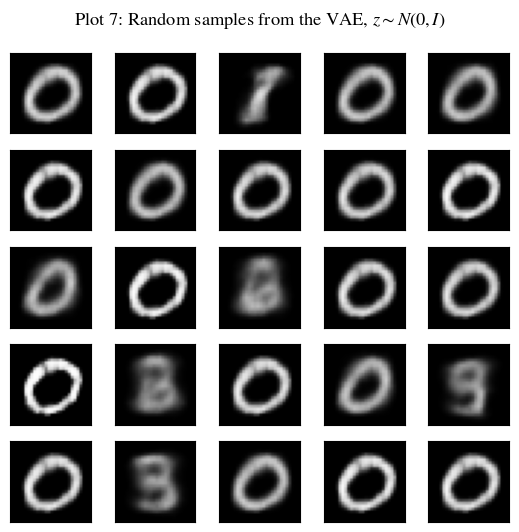
\includegraphics[width=0.65\textwidth]{cell31_img0.png}\caption{Randomly generated MNIST images from the VAE prior.}\label{fig:vaegen}\end{figure}

The generated samples demonstrate that the VAE can produce digit-like images from latent samples. Some samples are clearer than others, reflecting the probabilistic nature and limited two-dimensional latent capacity.

\subsection*{11.2 Latent-Space Interpolation}
For two latent vectors $z_A$ and $z_B$, interpolation was performed using
\[
z(\alpha)=(1-\alpha)z_A+\alpha z_B,\qquad \alpha\in[0,1].
\]
Values of $\alpha$ from 0 to 1 in steps of 0.1 were decoded.

\begin{figure}[H]\centering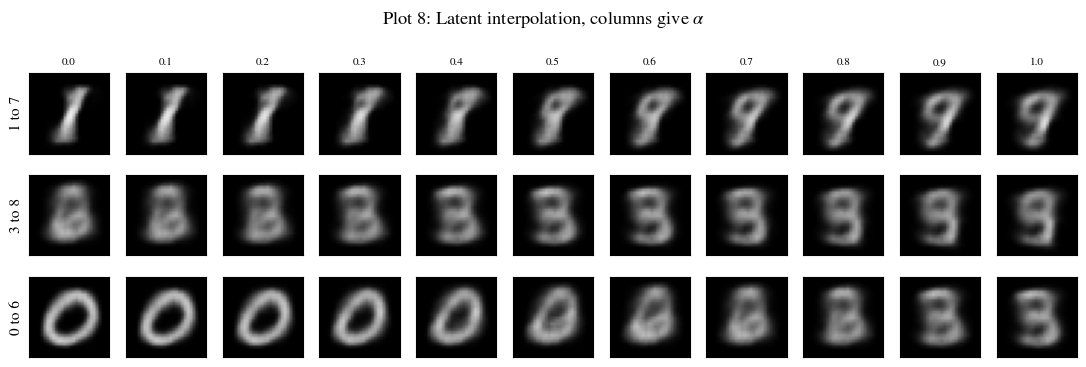
\includegraphics[width=0.6\textwidth]{cell32_img1.png}\caption{Latent-space interpolation examples.}\label{fig:interpolation}\end{figure}

The mean consecutive-frame MSE values were 0.0009 for the 1-to-7 pair, 0.0005 for 3-to-8 and 0.0020 for 0-to-6. The decoded images changed progressively between endpoints, demonstrating the continuous structure of the learned latent space.

\section*{12. Deterministic versus Probabilistic Latent Representations}
A separate FC-AE with $d_z=2$ was trained to compare a deterministic latent representation with the VAE latent space.

The FC-AE latent standard deviations were approximately $[13.72,10.43]$ with an auxiliary 5-NN accuracy of 0.588. The VAE latent standard deviations were approximately $[0.76,0.04]$ with 5-NN accuracy of 0.412.

\begin{figure}[H]\centering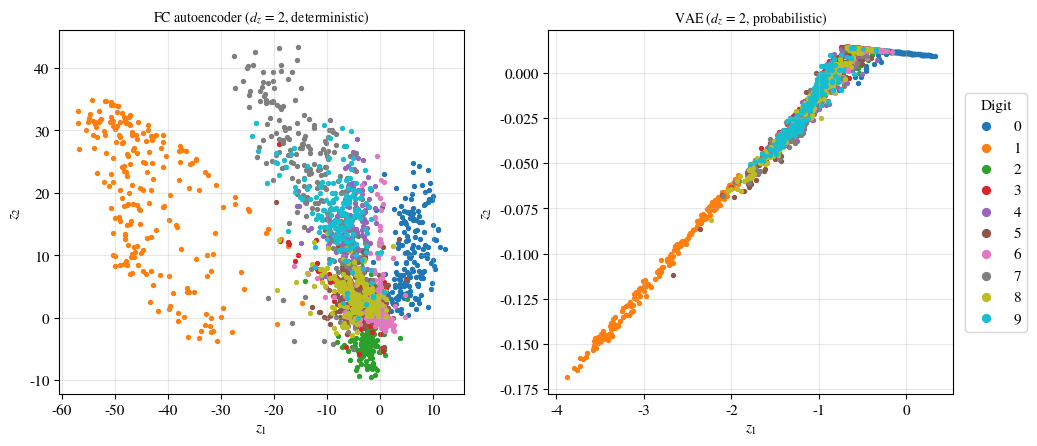
\includegraphics[width=0.90\textwidth]{cell33_img1.png}\caption{Comparison of deterministic FC-AE and probabilistic VAE latent spaces.}\label{fig:detprob}\end{figure}

The FC-AE learns a direct deterministic code for each image, whereas the VAE constrains the latent distribution toward a structured prior and supports sampling of new points.

\section*{13. Reconstruction Error Distribution}
For each test image, the reconstruction error was calculated as
\[
e_i=\frac{1}{D}\sum_{j=1}^{D}(x_{ij}-\hat{x}_{ij})^2.
\]
The resulting distributions were analyzed for the FC-AE, CAE and VAE.

\begin{center}
\begin{tabular}{lrrrrrrrr}
\toprule
Model & Mean & Median & SD & Min & P90 & P99 & Max & $>\mu+2\sigma$\\
\midrule
FC-AE & 0.01992 & 0.01894 & 0.01038 & 0.00184 & 0.03375 & 0.04822 & 0.07570 & 73\\
CAE & 0.00264 & 0.00243 & 0.00137 & 0.00039 & 0.00437 & 0.00724 & 0.01145 & 85\\
VAE & 0.05474 & 0.05496 & 0.01890 & 0.00513 & 0.07681 & 0.10548 & 0.14258 & 46\\
\bottomrule
\end{tabular}
\end{center}

\begin{figure}[H]\centering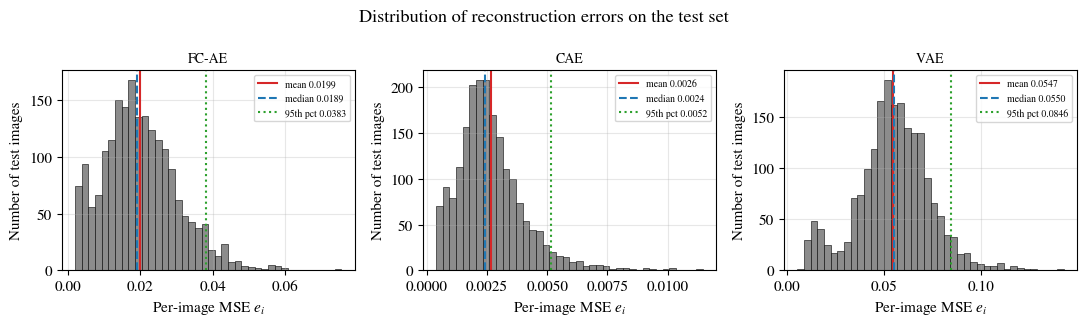
\includegraphics[width=0.90\textwidth]{cell35_img1.png}\caption{Distribution of per-image reconstruction errors.}\label{fig:errorhist}\end{figure}

The CAE has the lowest typical reconstruction error and a relatively concentrated error distribution. The VAE has a higher error distribution, consistent with the strong compression imposed by its two-dimensional probabilistic latent space.

\section*{14. High-Error Image Analysis}
The five highest-error samples were identified for each model. For the FC-AE, the largest-error samples included digit 5 (error 0.0757), digit 8 (0.0603 and 0.0592), digit 6 (0.0588) and digit 4 (0.0586). For the CAE, the largest errors ranged from 0.0093 to 0.0114. For the VAE, the five largest errors ranged from 0.1201 to 0.1426.

\begin{figure}[H]\centering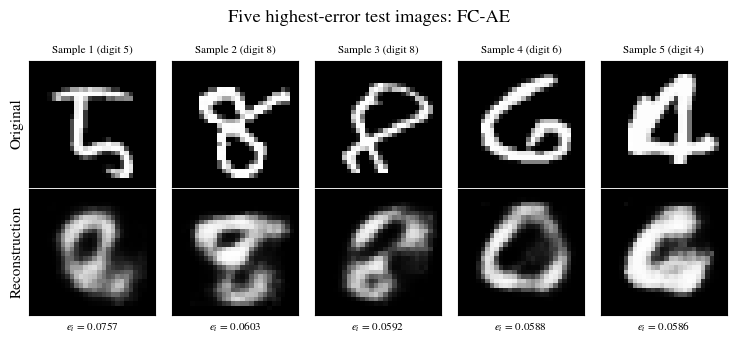
\includegraphics[width=0.95\textwidth]{cell36_img0.png}\caption{Highest-error examples for the FC-AE.}\label{fig:highfc}\end{figure}

\begin{figure}[H]\centering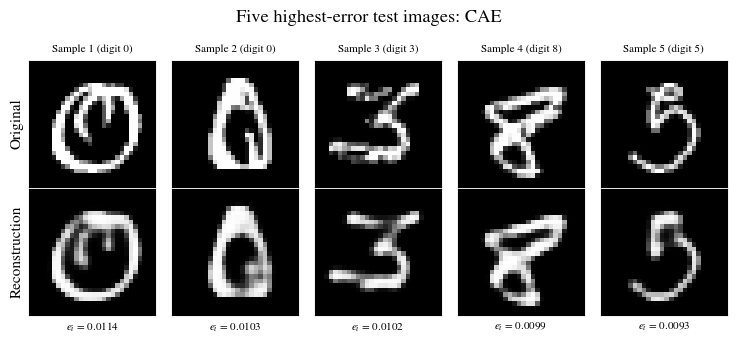
\includegraphics[width=0.95\textwidth]{cell36_img2.png}\caption{Highest-error examples for the convolutional autoencoder.}\label{fig:highcae}\end{figure}

\begin{figure}[H]\centering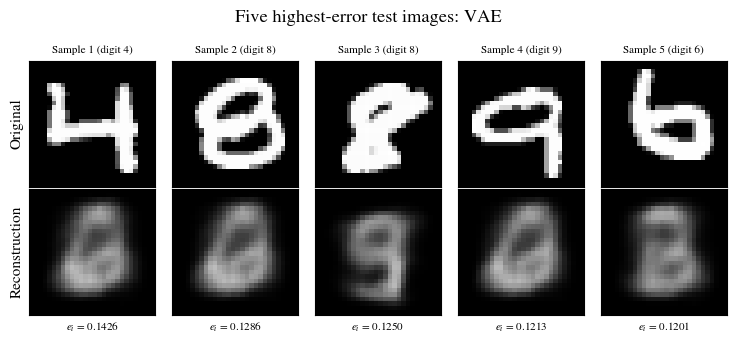
\includegraphics[width=0.95\textwidth]{cell36_img4.png}\caption{Highest-error examples for the VAE.}\label{fig:highvae}\end{figure}

The digit-wise analysis showed that digit 8 was the hardest class for the FC-AE and CAE, while digit 2 was hardest for the VAE. Digit 1 had the lowest mean reconstruction error for all three models. The Spearman correlation between error and total image intensity was 0.39 for FC-AE, 0.31 for CAE and 0.63 for VAE.

\section*{15. Consolidated Results}
\begin{center}
\begin{tabular}{lrrrrr}
\toprule
Model & MSE & MAE & SSIM & Parameters & Time (s)\\
\midrule
FC Autoencoder & 0.01992 & 0.05442 & 0.7749 & 211040 & 12.0\\
Conv. Autoencoder & 0.00264 & 0.01554 & 0.9725 & 74497 & 20.7\\
Denoising CAE & 0.00444 & 0.02111 & 0.9480 & 74497 & 17.8\\
VAE & 0.05474 & 0.12666 & 0.3661 & 134165 & 26.9\\
\bottomrule
\end{tabular}
\end{center}

The plain CAE achieved the lowest test MSE and highest mean SSIM among the reconstruction models in this execution. The denoising CAE also retained high structural similarity while handling corrupted inputs. The FC-AE was faster to train but used more parameters and produced larger reconstruction errors. The VAE had a different objective because its total loss includes KL divergence in addition to reconstruction loss.

\section*{16. Required Inferences}
\begin{itemize}
\item \textbf{Effect of latent dimension:} Increasing $d_z$ from 2 to 32 reduced MSE from 0.04718 to 0.01919 and increased SSIM from 0.4729 to 0.7814.
\item \textbf{FC-AE vs CAE:} The CAE preserved spatial locality and produced substantially lower reconstruction error with fewer parameters in this experiment.
\item \textbf{Gaussian noise:} Increasing $\sigma$ from 0.1 to 0.3 increased denoised MSE and MAE and reduced SSIM.
\item \textbf{Denoising ability:} The denoising CAE recovered major digit structure and improved all three reported metrics relative to the noisy inputs.
\item \textbf{VAE latent distribution:} The VAE organizes information in a probabilistic latent space constrained by KL divergence toward a standard normal prior.
\item \textbf{Latent-space structure:} The 2-D VAE representation contains overlapping digit regions, as reflected by the auxiliary 5-NN accuracy of 0.412.
\item \textbf{Generation:} Sampling from $\mathcal{N}(0,I)$ produced digit-like images with visible variation, although some generated samples were ambiguous.
\item \textbf{Interpolation:} Decoding linearly interpolated latent vectors produced gradual changes between selected endpoints.
\item \textbf{Reconstruction error and visual quality:} Higher per-image MSE generally corresponds to more visible reconstruction differences, motivating inspection of high-error samples.
\item \textbf{Deterministic vs probabilistic representation:} The FC-AE maps each input to a deterministic code, while the VAE learns distribution parameters and enables sampling and generation.
\end{itemize}

\section*{17. Conclusion}
The experiment demonstrated a complete progression from deterministic image reconstruction to denoising and probabilistic generative modeling. The fully connected autoencoder successfully learned compact representations, while the convolutional autoencoder substantially improved reconstruction quality by preserving spatial structure. The denoising CAE recovered meaningful digit structure from both Gaussian and salt-and-pepper corruption. The VAE learned a two-dimensional probabilistic latent space, generated new digit-like images and supported smooth latent interpolation. Overall, the results illustrate the different objectives and behavior of deterministic reconstruction models, denoising models and variational generative models.

\section*{18. References}
\begin{enumerate}
\item Ian Goodfellow, Yoshua Bengio and Aaron Courville, \textit{Deep Learning}, MIT Press, 2016.
\item Diederik P. Kingma and Max Welling, ``Auto-Encoding Variational Bayes,'' ICLR, 2014.
\item Pascal Vincent et al., ``Stacked Denoising Autoencoders: Learning Useful Representations in a Deep Network with a Local Denoising Criterion,'' Journal of Machine Learning Research, 2010.
\item Yann LeCun, Corinna Cortes and Christopher J. C. Burges, ``MNIST Handwritten Digit Database.''
\item TensorFlow Documentation: \url{https://www.tensorflow.org}
\item Keras Documentation: \url{https://keras.io}
\item scikit-image Documentation: \url{https://scikit-image.org}
\end{enumerate}

\vspace{10mm}

\begin{itemize}
    \item NAME: T Pranav Varshin(24110413)
    \item Reg No: 24011101116
    \item Section: AIDS-B
\end{itemize}


\end{document}
